\documentclass[hidelinks,11pt,dvipsnames]{article}
% xcolor commonly causes option clashes, this fixes that
\PassOptionsToPackage{dvipsnames,table}{xcolor}
\usepackage[tmargin=1in, bmargin=1in, lmargin=0.8in, rmargin=1in]{geometry}

%%%%%%%%%%%%%%%%%%%%%%%%%%%%%%%%%%%%%%%%%%%%%%%%%%%%%%%%%%%%%%%%%%%%
%%% For inkscape-figures
%%% Assumes the following directory structure:
%%% master.tex
%%% figures/
%%%     figure1.pdf_tex
%%%     figure1.svg
%%%     figure1.pdf
%%%%%%%%%%%%%%%%%%%%%%%%%%%%%%%%%%%%%%%%%%%%%%%%%%%%%%%%%%%%%%%%%%%%
%\usepackage{import}
\usepackage{pdfpages}
\usepackage{transparent}

\newcommand{\incfig}[2][1]{%
    \def\svgwidth{#1\columnwidth}
    \import{./figures/}{#2.pdf_tex}
}

\pdfsuppresswarningpagegroup=1

% enable synctex for inverse search, whatever synctex is
\synctex=1
\usepackage{float,macrosabound,homework,theorem-env}
\usepackage{microtype}


% font stuff
\usepackage{sectsty}
\allsectionsfont{\sffamily}
\linespread{1.1}

% bibtex stuff
\usepackage[backend=biber,style=alphabetic,sorting=anyt]{biblatex}
\addbibresource{main.bib}

% colored text shortcuts
\newcommand{\blue}[1]{\color{MidnightBlue}{#1}}
\newcommand{\red}[1]{\textcolor{Mahogany}{#1}}
\newcommand{\green}[1]{\textcolor{ForestGreen}{#1}}


% use mathptmx pkg while using default mathcal font
\DeclareMathAlphabet{\mathcal}{OMS}{cmsy}{m}{n}

% fixes the positioning of subscripts in $$ $$
\renewcommand{\det}{\operatorname{det}}

\usetikzlibrary{positioning, arrows.meta}
\newcommand{\here}[2]{\tikz[remember picture]{\node[inner sep=0](#2){#1}}}

%%%%%%%%%%%%%%%%%%%%%%%%%%%%%%%%%%%%%%%%%%%%%%%%%%%%%%%%%%%%%%%%%%%%%
%%% Entry Counter
%%%%%%%%%%%%%%%%%%%%%%%%%%%%%%%%%%%%%%%%%%%%%%%%%%%%%%%%%%%%%%%%%%%%%
\newcounter{entry-counter}
\newcommand{\entry}[1]
{
	\addtocounter{entry-counter}{1}
    \tchap{Entry \arabic{entry-counter}}
	%\addcontentsline{toc}{section}{Entry \arabic{entry-counter}: #1}
	\vspace{-1.5em}
    \begin{center}
		\small \emph{Written: #1}
    \end{center}
}

\usepackage{titling}
\renewcommand\maketitlehooka{\null\mbox{}\vfill}
\renewcommand\maketitlehookd{\vfill\null}


\usepackage{capt-of}
\usepackage{tikz}
\usetikzlibrary{positioning,calc,intersections,through,backgrounds, shapes.geometric, decorations.markings,arrows}

\def\sset{\subseteq}
\def\iso{\cong}
\def\gend#1{\langle #1\rangle}

\newcommand{\rightoverleftarrow}{%
  \mathrel{\vcenter{\mathsurround0pt
    \ialign{##\crcr
      \noalign{\nointerlineskip}$\longrightarrow$\crcr
      \noalign{\nointerlineskip}$\longleftarrow$\crcr
    }%
  }}%
}

\newcommand\makesphere{} % just for safety
\def\makesphere(#1)(#2)[#3][#4]{%
  % Synopsis
  % \makesphere[draw options](center)(initial angle:final angle:radius)
  \shade[ball color = #3, opacity = #4] #1 circle (#2);
  \draw #1 circle (#2);
  \draw ($#1 - (#2, 0)$) arc (180:360:#2 and 3*#2/10);
  \draw[dashed] ($#1 + (#2, 0)$) arc (0:180:#2 and 3*#2/10);
}
% same thing as makesphere but places white background behind
\newcommand\altmakesphere{} % just for safety
\def\altmakesphere(#1)(#2)(#3)[#4][#5]{%
  % Synopsis
  % \make sphere[draw options](center)(initial angle:final angle:radius)
  \draw [fill=white!30] #1 circle (#2);
  \shade[ball color = #4, opacity = #5] #1 circle (#2);
  \draw #1 circle (#2);
  \draw ($#1 - (#2, 0)$) arc (180:360:#2 and 3*#2/10);
  \draw[dashed] ($#1 + (#2, 0)$) arc (0:180:#2 and 3*#2/10);
  \node at #1 {#3};
}

\begin{document}
% set section number to 1
% fixes theorem numbering without need to have a section title
\setcounter{section}{1}

\pagestyle{empty}
	\LARGE
\begin{center}
	Algebraic Topology Homework 9 \\
	\Large
	Isaac Martin \\
    Last compiled \today
\end{center}
\normalsize
\vspace{-4mm}
\hru

\tchap{Problems from 2.2}
\begin{homework}[e]
  \prob[\textsc{Exercise 2.}] Given a map $:S^{2n}\to S^{2n}$ show that there is some point $x \in S^{2n}$ with either $f(x) = x$ or $f(x) = -x$. Deduce that every map $\bRP^{2n}\to \bRP^{2n}$ has a fixed point. Construct maps $\bRP^{2n - 1}\to \bRP^{2n - 1}$ without fixed points from linear transformations $\bRP^{2n}\to \bRP^{2n}$ without eigenvectors.
  \begin{prf}
    It suffices to show that either $f$ or $-f$ has a fixed point, for if $f$ has a fixed point we're done and if $-f$ has a fixed point $a$ then $f(a) = -a$. Suppose first that $f$ has no fixed point. Then by property (g) of degree on page 134 of Hatcher, $\deg(f) = (-1)^{2n + 1} = -1$. If $-f$ has no fixed pint, then it too has degree $-1$ for the same reason, but this is not possible since $-f$ is $f$ composed with a reflection $r$, and hence must satisfy $\deg(-f) = \deg(r\circ f) = \deg(r)\circ \deg(f) = -\deg(f)$. Thus, at least one of $f$ and $-f$ has a fixed point.

    Now consider a map $f:\bRP^{2n}\to \bRP^{2n}$. The space $S^{2n}$ is a simply connected cover of $\bRP^{2n}$. By the lifting criterion, we therefore get a map $\tilf:S^{2n}\to S^{2n}$ such that $p\circ \tilf = f\circ p$, where $p:S^{2n}\to \bRP^{2n}$ is the covering map, which is simply the quotient map $S^{2n}\to S^{2n}/\sim = \bRP^{2n}$ where $x \sim -x$. Let $x$ be a point such that $\tilf(x) = - x$ or $\tilf(x) = x$, which must exist by what we have already shown. Then $p\circ \tilf(x) = p(\pm x) = [x] = f(p(x)) = f([x])$. Here we have used $[x]$ to denote the coset of $x$ in $\bRP^{2n}$. Thus, $[x]$ is a fixed point of $f$.

    Consider a rotation of $\bR^{2n}$ given by multiplication by the matrix $A \in \SL_{2n}(\bR)$. Since $A$ is necessarily an isometry of $\bR^{2n}$, it maps $S^{2n-1}$ to $S^{2n-1}$. Suppose we had some $x \in S^{2n-1}$ fixed under multiplication by $A$. Then we would have $Ax = x$ and hence $1$ would be an eigenvalue of $A$, which can't happen since $A$ doesn't have any real eigenvalues. Likewise, if $Ax = -x$, then $-1$ would be an eigenvalue of $A$ which is similarly impossible. Hence, the rotation map given by $A$ on $S^{2n-1}$ is an example of a map on an odd-dimension sphere with neither fixed nor antipodal points.
  \end{prf}
  \prob[\textsc{Exercise 8.}] A polynomial $f(z)$ with complex coefficients, viewed as a map $\bC\to \bC$, can always be extended to a continuous map of one-point compactifications $\hatf:S^2 \to S^2$. Show that the degree of $\hatf$ equals the degree of $f$ as a  polynomial. Show also that the local degree of $\hatf$ at a root of $f$ is the multiplicity of the root.
  \begin{prf}
    Recall that any polynomial $f:\bC\to \bC$ can be written $f(z) = c(z - a_1)^{d_i}\cdot ... \cdot (z - a_k)^{d_k}$ where $a_1,...,a_k\in \bC$ are the roots of $f$ and $d_1 + ... + d_k = \deg f$. Let $\hatf$ denote the map induced on $S^2$ by $f$, and notice that by Proposition 2.30, the degree of $\hatf_*$ is equal to the sum of $\deg \hatf_* | a_i$, that is, the total degree of $\hatf_*$ can be found by summing the degrees of $\hatf_*$ restricted to small neighborhoods of its zeros. Note also that the extension of $f$ to the Riemann sphere is given by sending $\infty \mapsto \infty$, i.e. on any open set $U$ of the Riemann sphere \emph{not} containing $\infty$, $\hatf|_U = f|_U$.

    For each root $a_i$ we may find an open disk $U_i$ containing $a_i$ which doesn't contain $\infty$ or any other roots of $f$. Because $f$ is a polynomial, it is holomorphic and hence has a convergent Taylor series in $U_i$, provided we choose $U_i$ to be small enough. This means that for $z \in U_i$,
    \begin{align*}
      \hatf(z) = (z - a_i)^{d_i}(c_0 + c_1(z-a_i) + c_2(z-a_i)^2+...).
    \end{align*}
    Let $V$ be a neighborhood of $0$ such that $\hatf(U_i) = f(U_i) \subseteq V$ for all $1\leq i\leq k$. Near a root $a_i$, $c_0(z - a_i)^{d_i}$ is a good approximation for $\hatf(z)$, i.e. for a sufficiently small circle $S_r(a_i)\subseteq \bC$ of radius $r$ centered at $a_i$ parameterized by $\gamma:[0,1]\to S_r(a_i)$, $\hatf\circ \gamma$ will wrap around the circle $S_{c_0r}(0)$ $d_i$ times, potentially with some perturbation/wobble. This means the local degree of $\hatf_*$ at $a_i$ is $d_i$, since $\hatf$ and $f$ are equal when restricted to $U_i$. Applying Proposition 2.30, we see that
    \begin{align*}
      \deg \hatf_* = \sum_{i=1}^k \deg \hatf_*|_{U_i} = d_1 + ... + d_k = \deg f,
    \end{align*}
    where $\deg f$ is the degree of $f$ as a polynomial. This gives us good reason to call the degree of a map $S^n \to S^n$ ``degree'' in the first place.
    \begin{center}
      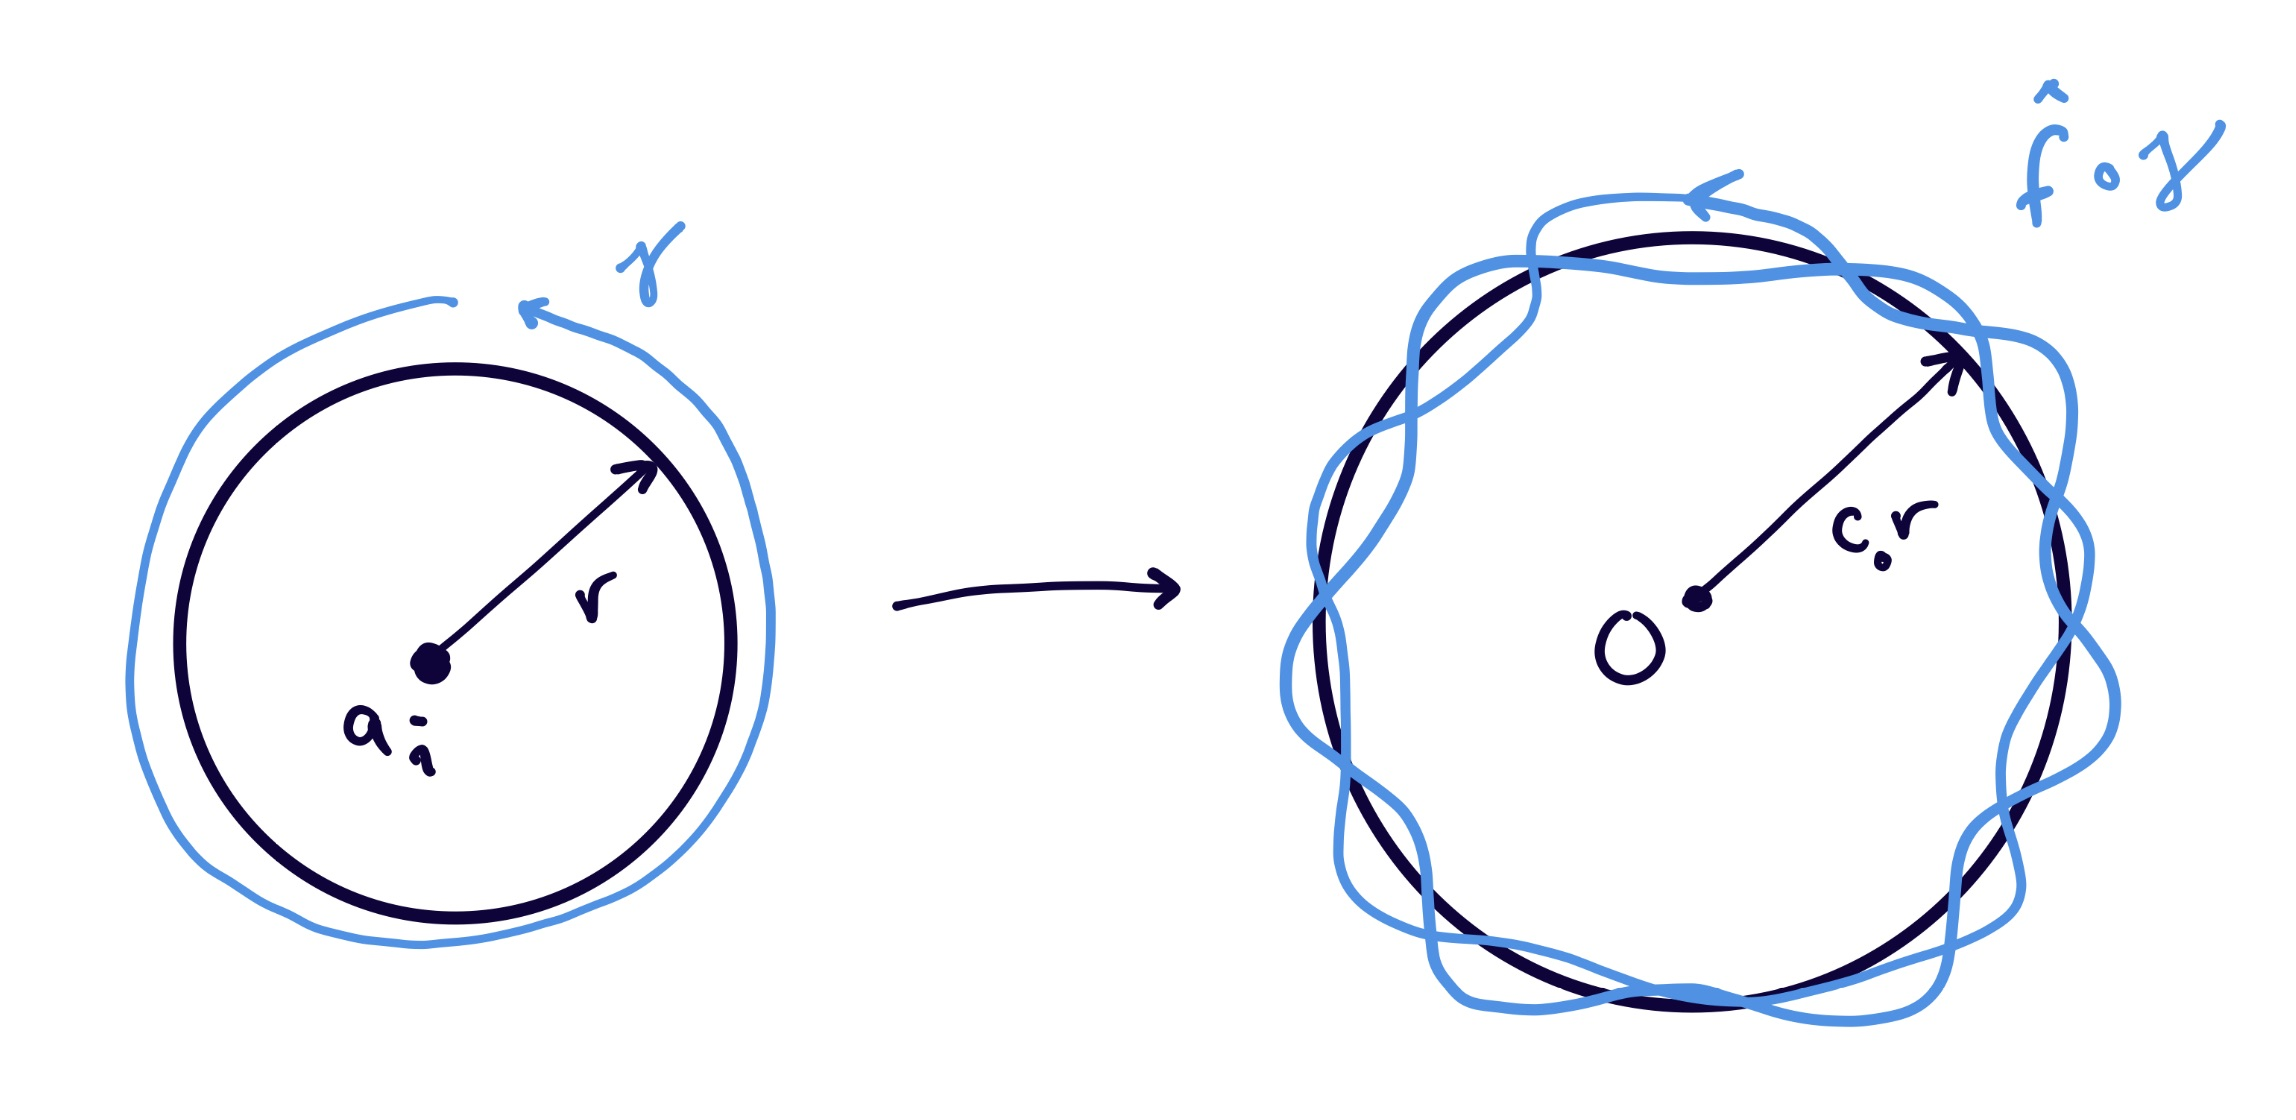
\includegraphics[width=12cm]{figures/hwk10-fig1.png}
      \captionof{figure}{The map $\hatf \circ \gamma$ is $c_0(z - a_i)^{d_i}$ plus some wobble.}
      \label{fig:prob1-1}
    \end{center}
  \end{prf}
  \prob[\textsc{Exercise 9.}] Compute the homology groups of the following $2$-complexes.
  \begin{enumerate}[(a)]
    \item The quotient of $S^2$ obtained by identifying the north and south poles to a point.
    \item $S^1\times (S^1\vee S^1)$
    \item The space obtained from $D^2$ be first deleting the interiors of two disjoint subdisks in the interior of $D^2$ and then identifying all three resulting boundary circles together via homeomorphisms preserving clockwise orientations of these circles.
    \item The quotient space of $S^1\times S^1$ obtained by identifying points in the circle $S^1\times \{x_0\}$ that differ by $2\pi/m$ rotation and identifying points in the circle $\{x_0\}\times S^1$ that differ by $2\pi/n$ rotation.
  \end{enumerate}
  \begin{prf}
    \begin{enumerate}[(a)]
      \item I'm likely ``supposed'' to use cellular homology, but this space is homotopy equivalent to $S^2$ together with a diameter running from the north to south pole (simply contact the diameter to a point to get the equivalence). We previously showed that this space is homotopy equivalent to $S^2 \vee S^1$ with the following picture to support our argument:
    \begin{center}
      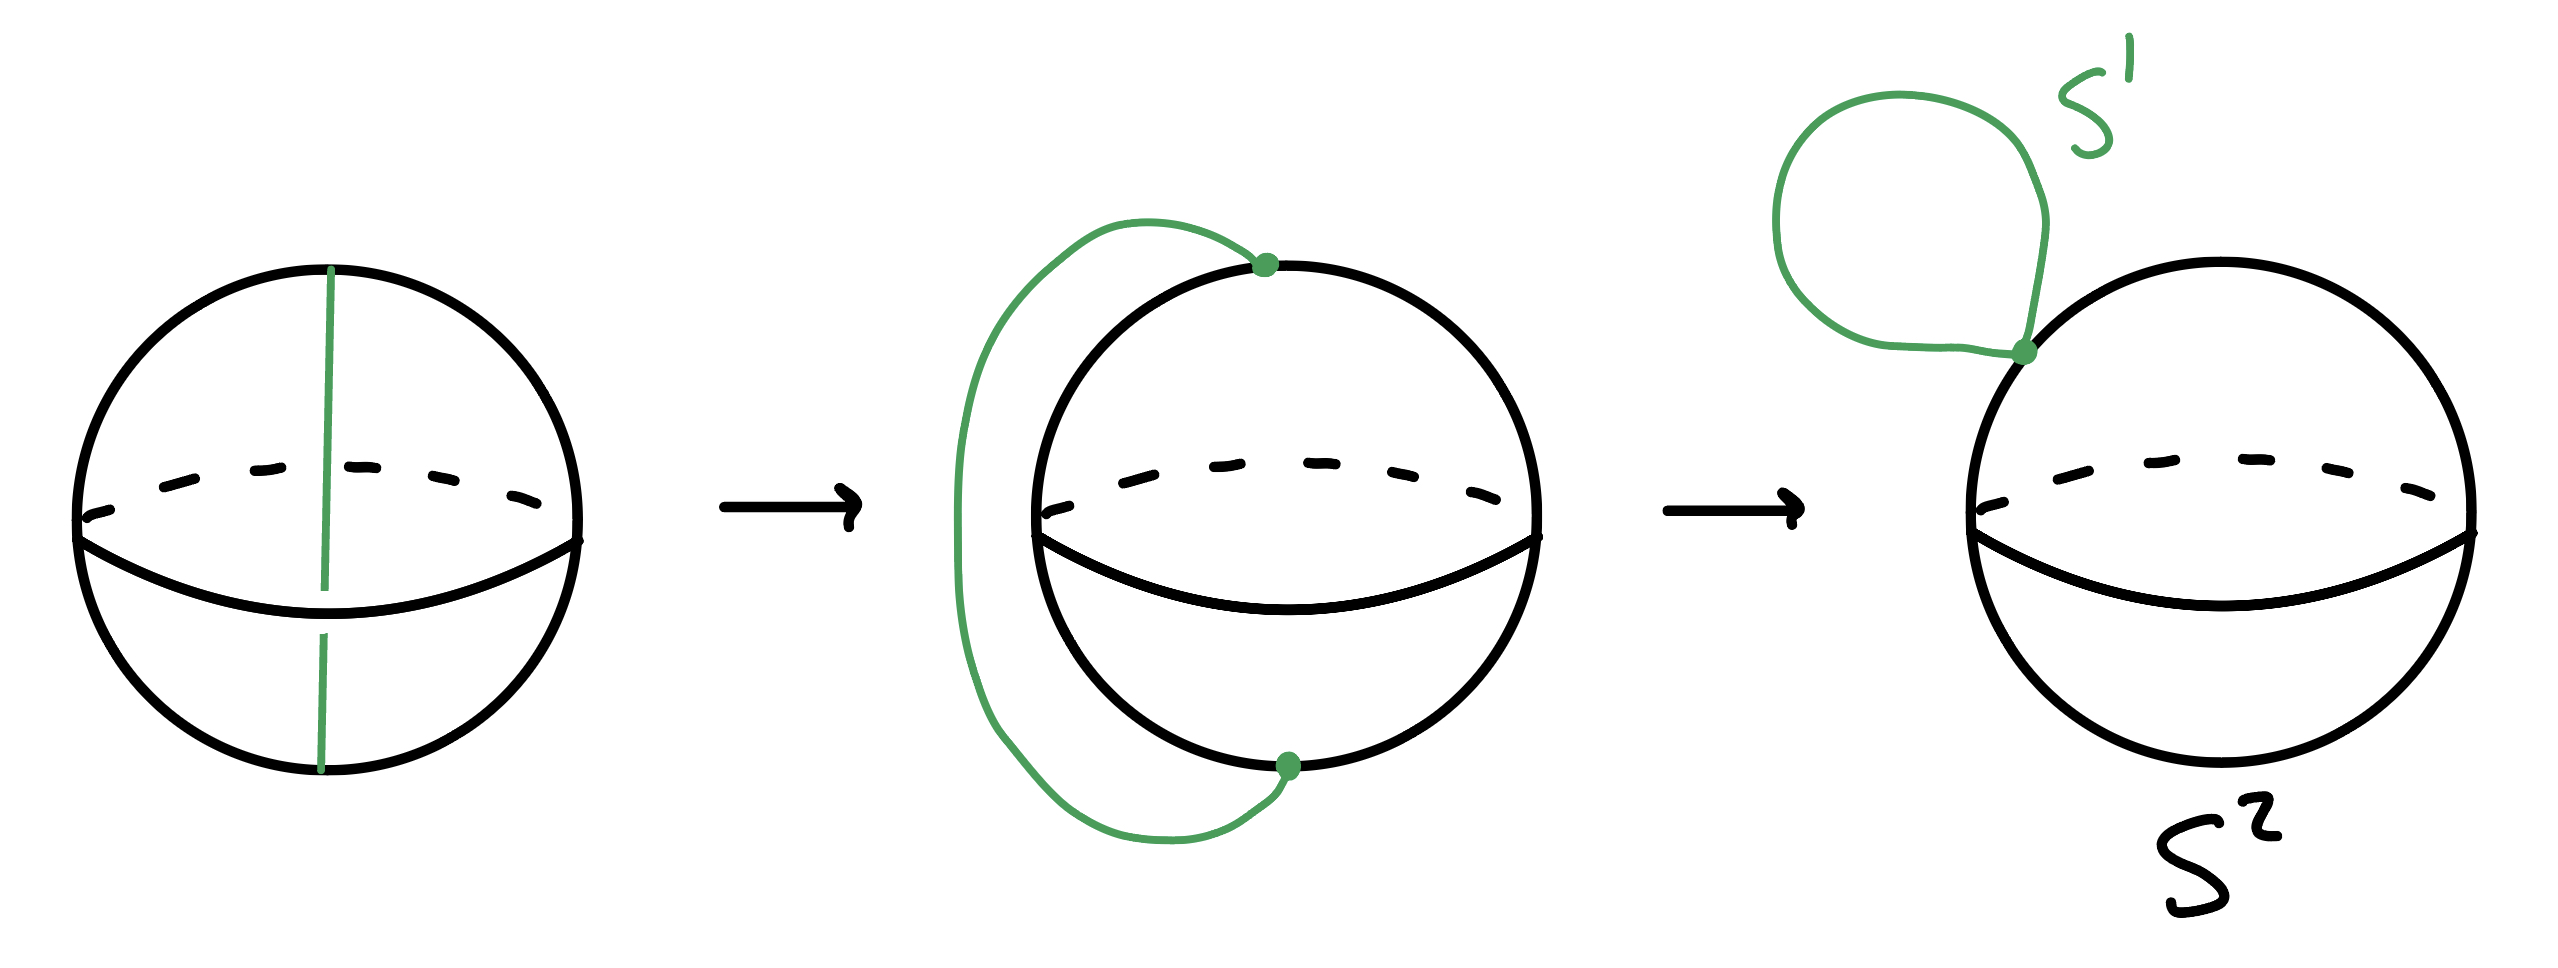
\includegraphics[width=12cm]{figures/hwk5-fig5.jpg}
      \captionof{figure}{$S^2$ together with a line segment connecting the north and south pole is homotopy equivalence to $S^2\vee S^1$}
      \label{fig:prob9-1}
    \end{center}
    Since $(S^2,\{p\})$ and $(S^2,\{p\})$ are good pairs, where $p$ is the wedge point, we have that
    \begin{align*}
      \tilH_i(S^2\vee S^1) = \tilH_i(S^2) \oplus \tilH_i(S^1).
    \end{align*}
    Letting $X$ be the original space in question, we have
    \begin{align*}
      H_i(X) =
      \begin{cases}
        \bZ & i = 0,1,2 \\
        0 & \text{else}
      \end{cases}
    \end{align*}
    \item Let $X = S^1 \times (S^1 \vee S^1)$. This is equivalent to $I\times (S^1\vee S^1)$ with the endpoints $\{0\}\times (S^1\vee S^1)$ and $\{1\}\times (S^1\vee S^1)$ identified, or in other words, two tori identified at one of their outer circles.
    \begin{center}
      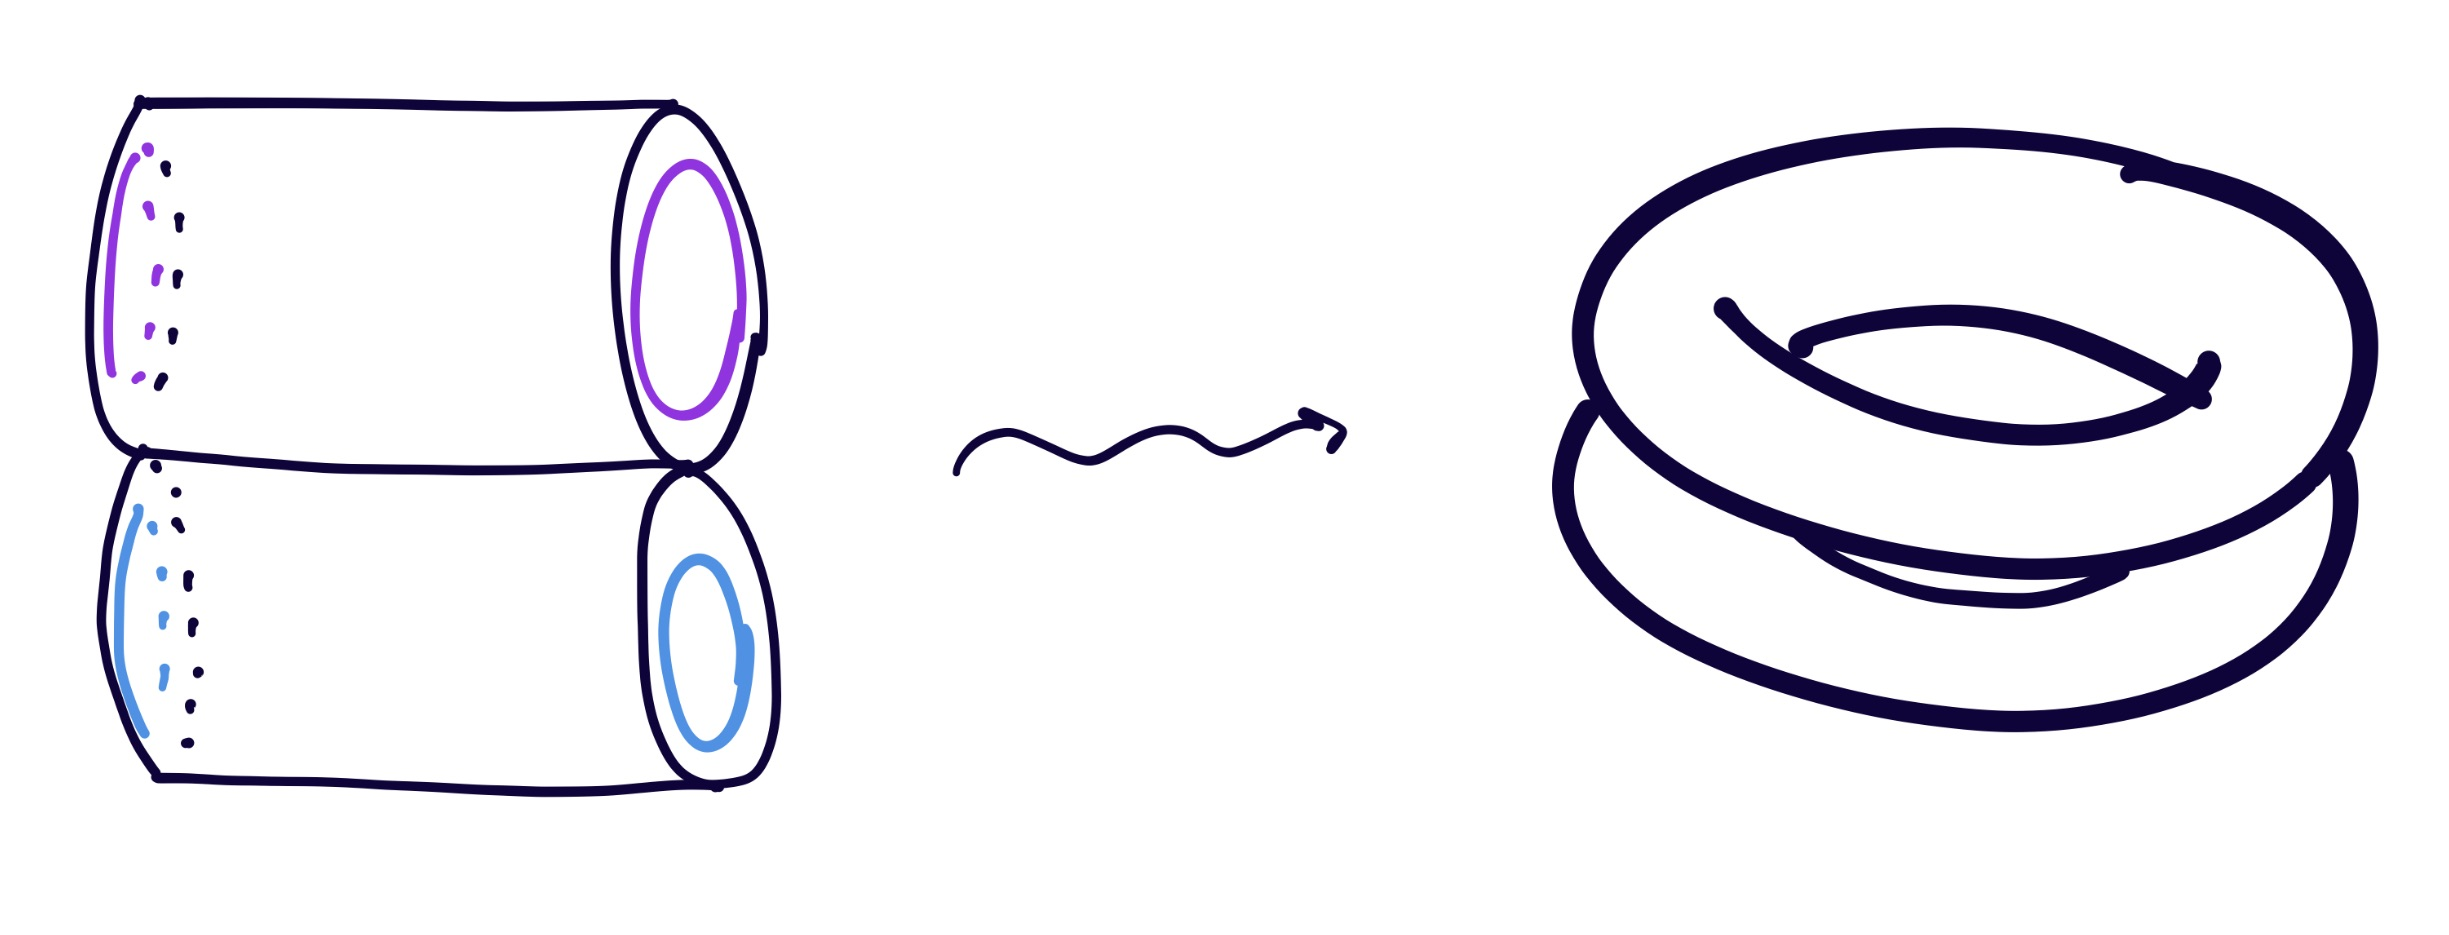
\includegraphics[width=12cm]{figures/hwk12-fig1.png}
      \captionof{figure}{The space $S^1\times (S^1\vee S^1)$}
      \label{fig:prob9-300}
    \end{center}
      We define $A = S^1 \times (S^1 \times U)$ and $B = S^1 \times (V \vee S^1)$ where $U$ and $V$ are small neighborhoods of the wedge point $x_0$ in their respective circles. Since $A$ and $B$ deformation retract to tori, we consider them to be tori without changing the homology groups. $A \cap B = S^1$, and we therefore have
        \begin{equation*}
        H_n(A\cap B) = 
        \begin{cases}
            \bZ & n=0,1 \\
            0 & \text{else} \\
        \end{cases}
        \hspace{2em}
        H_n(A) = 
        \begin{cases}
            \bZ & n=0,2 \\
            \bZ^2 & n=1 \\
            0 & \text{else} \\
        \end{cases}
        \hspace{2em}
        H_n(B) = 
        \begin{cases}
            \bZ & n=0,2 \\
            \bZ^2 & n=1 \\
            0 & \text{else} \\
        \end{cases}
        \hspace{3em}
      \end{equation*}
      for our homology groups. Mayer-Vietoris says that the following is an exact sequence:
      \begin{center}
          \begin{tikzcd}[cramped ,sep=small]
          0 \arrow[r]& H_3(X) \arrow [r, "\partial_3"]& 0 \arrow [r, "\Phi_2"]& \bZ\oplus\bZ \arrow[r,r, "\Psi_2"]& H_2(X) \arrow[r,"\partial_2"]& \bZ \arrow[r,"\Phi_1"]& \bZ^2\oplus\bZ^2 \arrow[r, r, "\Psi_1"]& H_1(X) \arrow[r, "\partial_1"]& ... \\
                     & & & ...~\bZ \arrow[r, "\Phi_0"]& \bZ^2 \arrow[r, "\Psi_0"]& H_0(X) \arrow[r, "\partial_0"] & 0
          \end{tikzcd}
      \end{center}
      Straight away we see that $H_3(X) = 0$ and that $H_0(X) = \bZ$ (which we could have seen from the reduced homology anyways). The details of this are discussed in problem 28 (a). 

      \medskip

      For $H_1(X)$ we first note that since $\Phi_0$ is injective, $\partial_1 = 0$. This means $\img\Psi_1 = \ker\partial_1 = H_1(X)$, so $\Psi_1$ is surjective. The map $\Phi_1$ is the map $x \mapsto (x,0,-x,0)$, since it takes a cycle in $A\cap B$ to its inclusion in $A$ and its inverse inclusion in $B$. The image of this is isomorphic to $\bZ$, and since $\ker\Psi_1 = \img\Phi_1 \cong \bZ$, the first isomorphism theorem tells us that $H_1(X) \cong \bZ$. Finally, $\partial_2$ is once again the zero map which makes $\Psi_2$ surjective. Since $\Phi_1$ is the inclusion of $0$ in $H_2(A) \oplus H_2(B)$, we know that $\Psi_2$ is an isomorphism. We conclude that 
      \begin{equation*}
          H_n(X) = 
          \begin{cases}
              \bZ^2 & n = 2 \\
              \bZ^3 & n = 1 \\
              \bZ^1 & n = 0 \\
              0 & \text{else}
          \end{cases}. 
      \end{equation*}

    \item Set $X$ equal to the space in question. Figure \ref{fig:prob9-2} shows a CW complex for this space.
      \begin{center}
        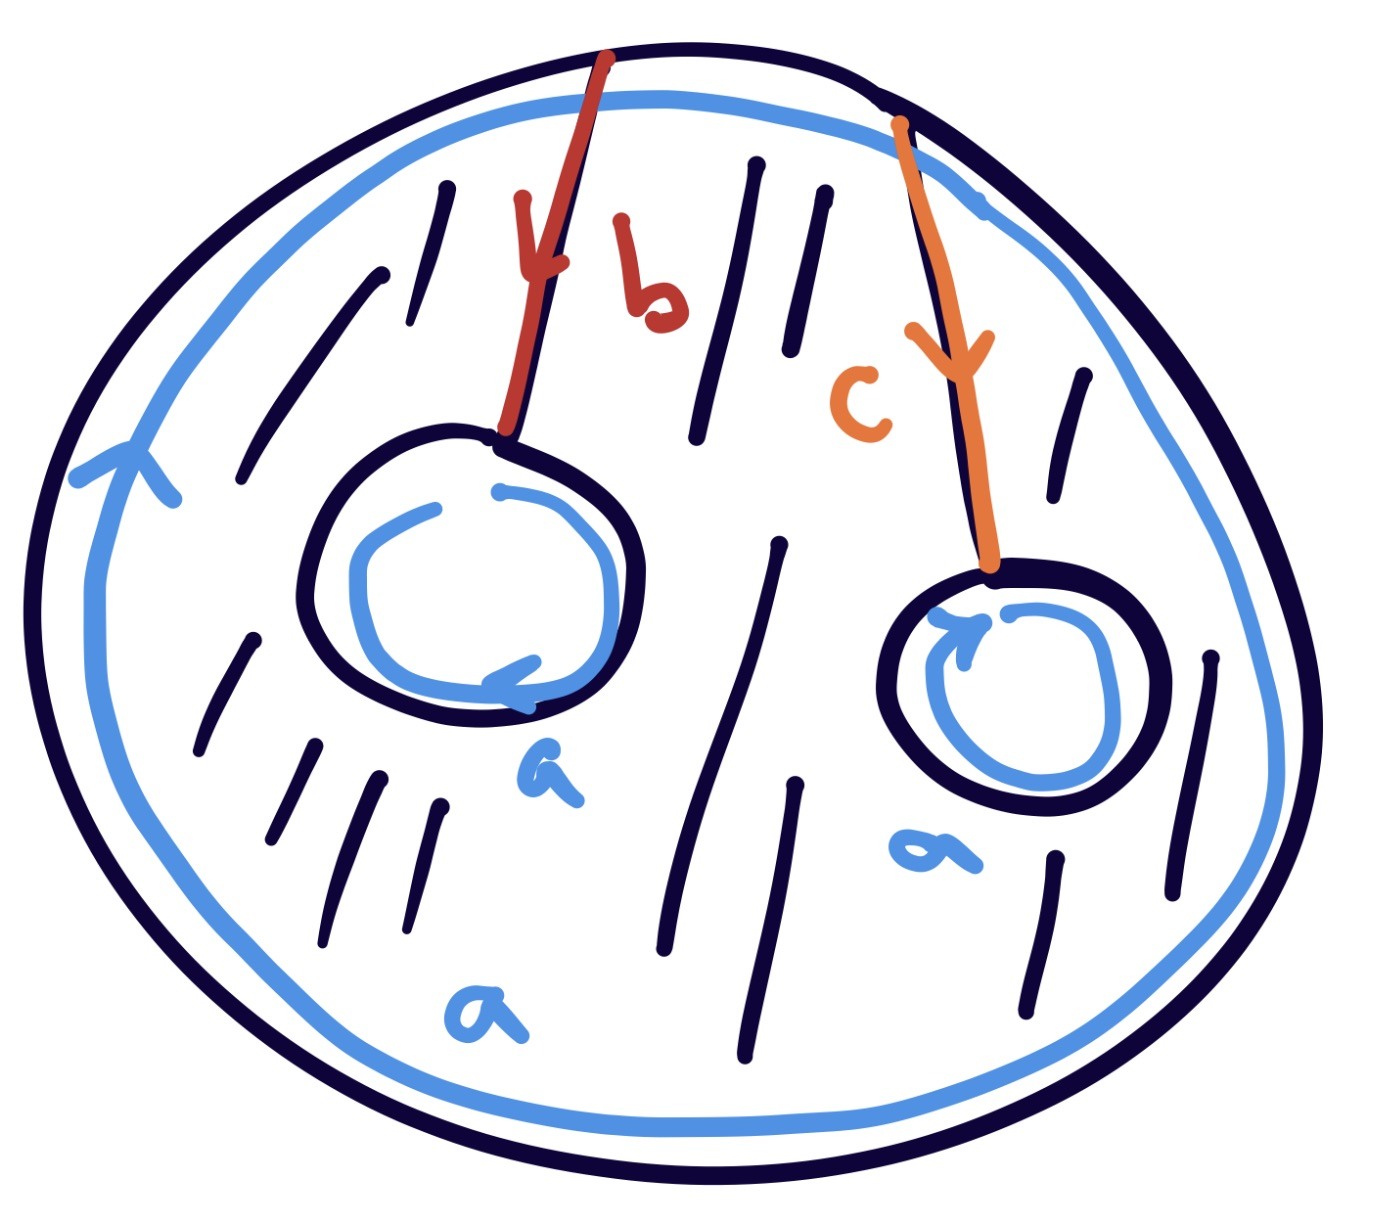
\includegraphics[width=5cm]{figures/hwk12-fig2.png}
        \captionof{figure}{CW complex of the space in 9 (c).}
        \label{fig:prob9-2}
      \end{center}
      Since there is one 2-cell, three 1-cells and one 0-cell the chain complex is
      \begin{align*}
        ... \to 0 \to \bZ \xrightarrow{\partial_2} \bZ^3 \xrightarrow{\partial_1} \bZ \to 0.
      \end{align*}
      Since the space is path connected, $H_0(X) = \bZ$. This implies that $\img \partial_1 = 0$, since $\bZ = \ker \partial_0/\img \partial_1 = \bZ/\img\partial_1$. Hence, we need only determine $\partial_2$, which entails checking its action on our single 2-cell. Call this 2-cell $f$. Since $C_1 \cong \bZ^3$ is generated by the 1-cells $[a]$, $[b]$ and $[c]$, we have that
      \begin{align*}
        \partial_2([f]) = x[a] + y[b] + z[c]
      \end{align*}
      for undetermined coefficients $x,y$ and $z$. These can be determined from the attaching map, drawn in figure \ref{fig:prob9-3}.
      \begin{center}
        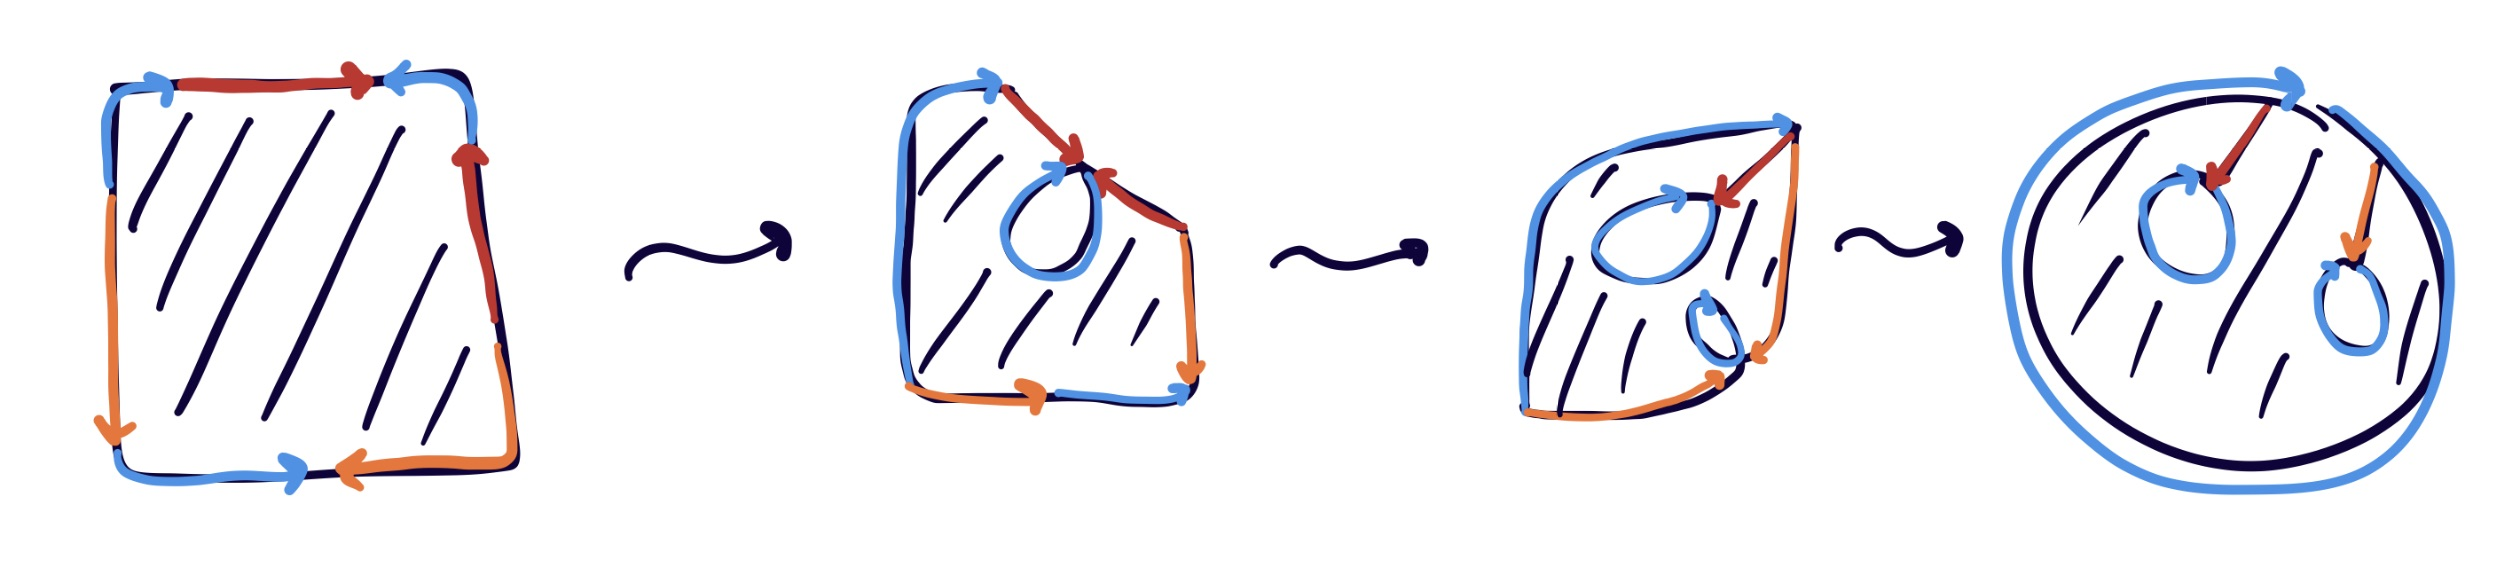
\includegraphics[width=12cm]{figures/hwk12-fig3.png}
        \captionof{figure}{Attaching map of the 2-cell to the 1-skeleton of $X$ in $9 (c)$}
        \label{fig:prob9-3}
      \end{center}
      To find $x$, we do the whole ``look at the image of the boundary in the crushed 1-skeleton where everything but $a$ is crushed'' thing, and then look at the degree. This amounts to traveling along the boundary of the square and counting all appearances of $a$ with sign, which gives us $1$ if you believe clockwise orientation should be negative (it definitely should be). Similarly, we get that $y = z = 0$ since both the red and orange arrows appear twice with each copy having opposite orientation. Thus,
      \begin{align*}
        \partial_2([f]) = [a],
      \end{align*}
      and we get the $\ker \partial_2 = 0$ and $\img\partial_2 = \bZ$. This means
      \begin{align*}
        H_i(X) =
        \begin{cases}
          \bZ & i = 0\\
          \bZ^2 & i = 1 \\
          0 & \text{otherwise}
        \end{cases}.
      \end{align*}
    \item The quotient space $X$ in question amounts to partitioning the typical cell complex structure on $T^2$ into $mn$ regions. It results in the usual rectangle of a 2-cell being split up into $mn$ smaller rectangles, seen in figure \ref{fig:prob9-4}.
      \begin{center}
        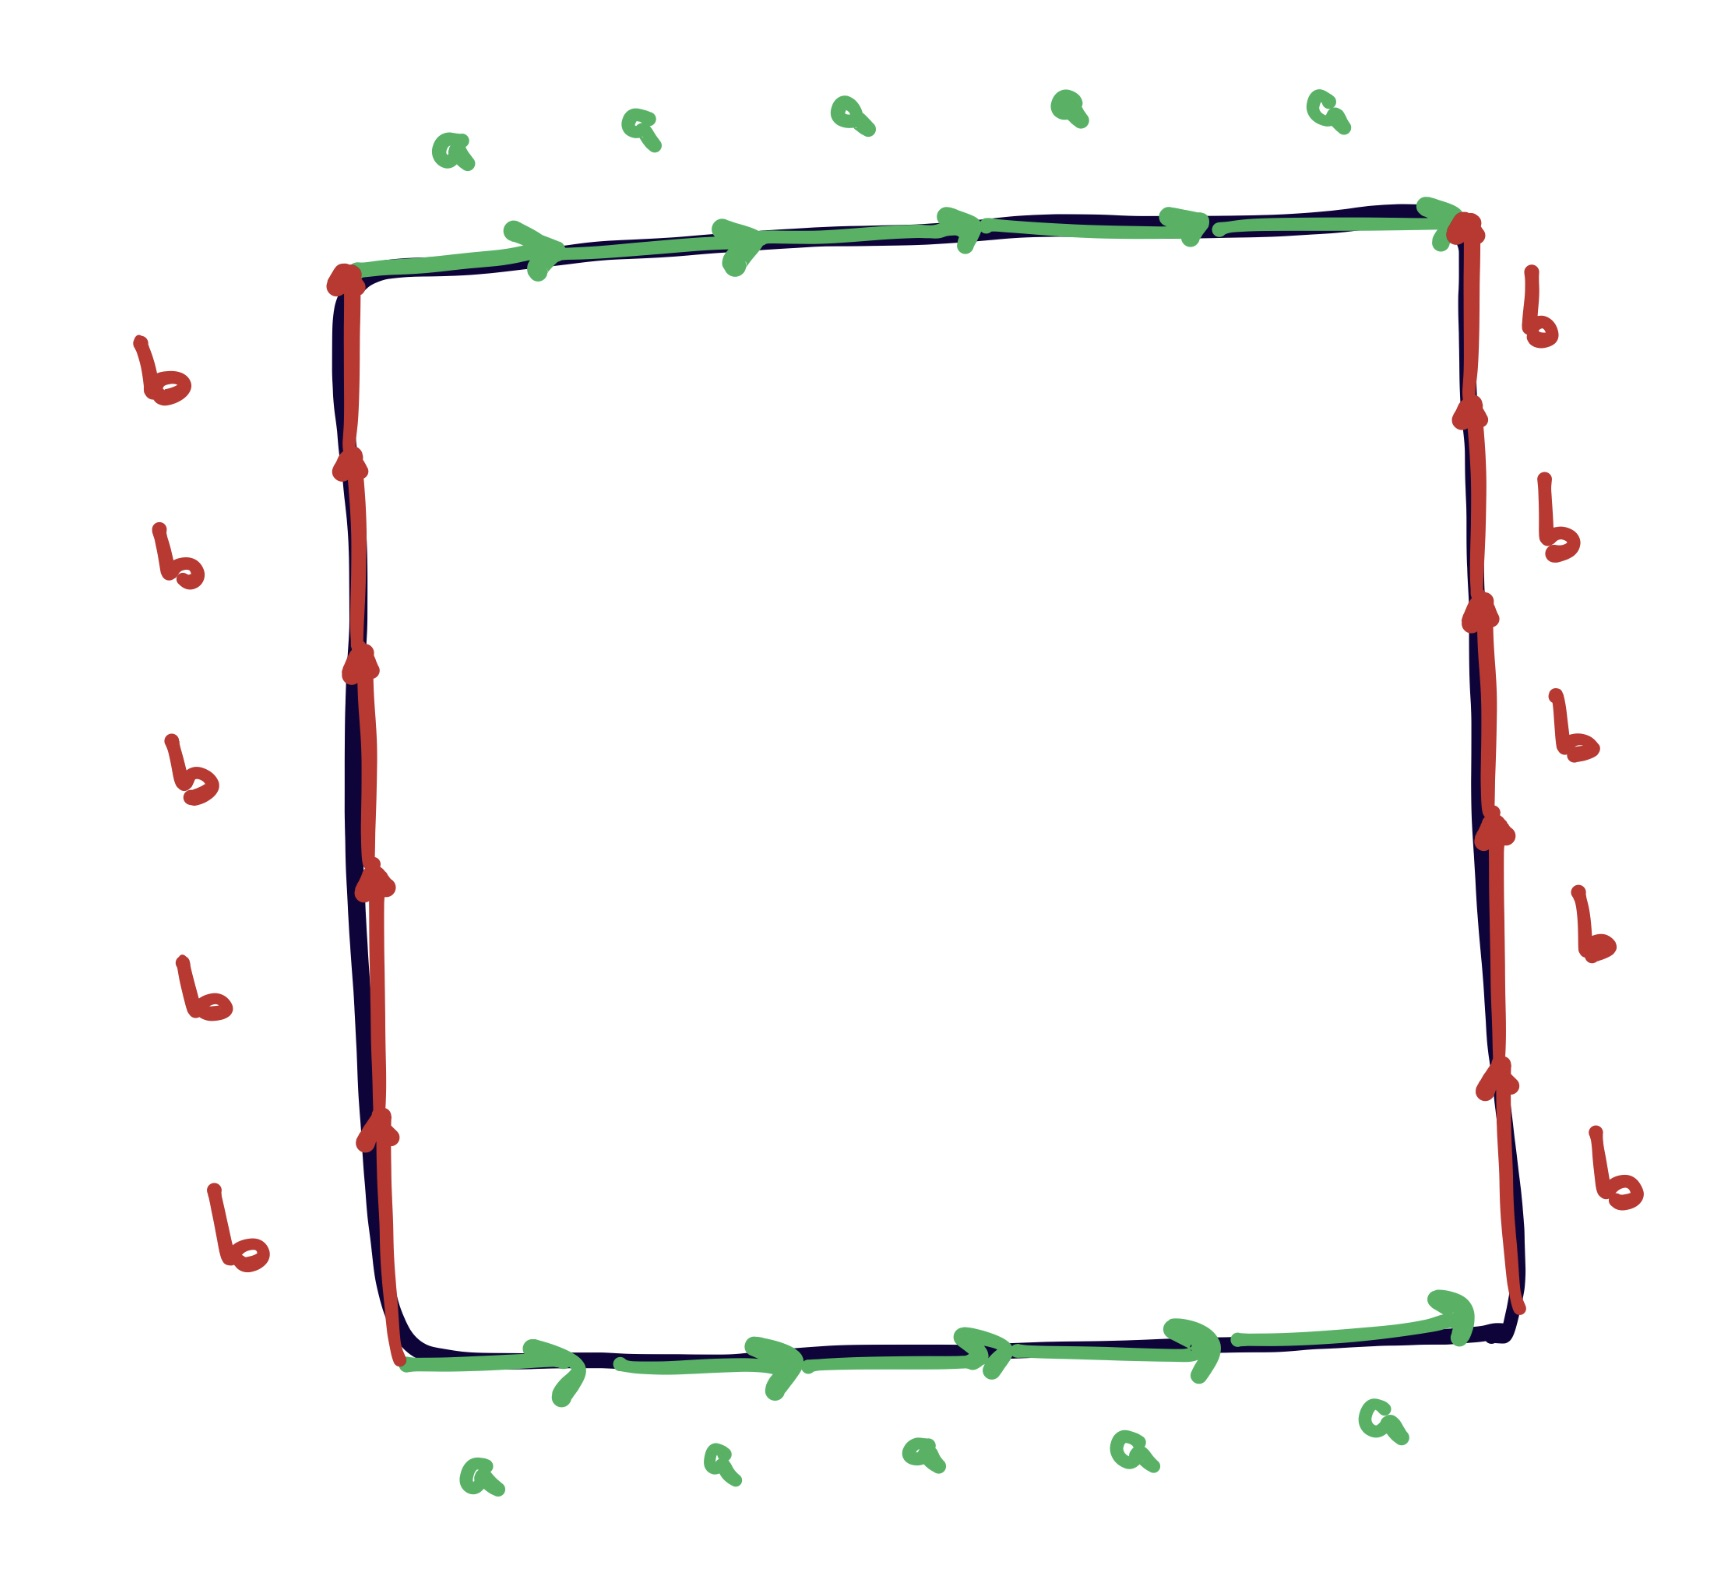
\includegraphics[width=12cm]{figures/hwk12-fig4.png}
        \captionof{figure}{Cell structure on the space in question in problem 9 (d)}
        \label{fig:prob9-4}
      \end{center}
    \end{enumerate}
    There is still only one 2-cell, two 1-cells, and one 0-cells, giving us a chain complex
    \begin{align*}
      ...\to 0\to \bZ \to \bZ^2 \to \bZ \to 0.
    \end{align*}
    The space is path connected as in part (c), so $\partial_1 = 0$ again. We also see that $\partial_2 = 0$ since the attaching map attaches $a$ to itself $m$ times in one direction and $m$ times in the other; similarly for $b$. Hence, all the chain maps are zero and the homology is simply the chain complex:
    \begin{align*}
      H_i(X) =
      \begin{cases}
        \bZ & i = 0,2 \\
        \bZ^2 & i = 1 \\
        0 & \text{otherwise}
      \end{cases}.
    \end{align*}
  \end{prf}
  \prob[\textsc{Exercise 10.}] Let $X$ be the quotient space of $S^2$ under the identifications $x \sim -x$ for $x$ in the equator $S^1$. Compute the homology groups $H_i(X)$. Do the same for $S^3$ with antipodal points of the equatorial $S^2 \subseteq S^3$ identified.
  \begin{prf}
    The identification along the equator produces a copy of $\bRP^1$ embedded inside $X$. We can put a cell structure on $X$ using this fact. Recall that we can construct $S^2$ as two disks with boundaries glued to a copy of $S^1$, in which case we get one disk each for the northern and southern hemisphere and the equator gets its very own 1-cell. This same procedure gives us a cell structure on $X$, but our gluing maps replicate the identification $x \sim -x$. In total, we use one 0-cell, one 1-cell and two 2-cells.

    We can regard $\bRP^1$ as traversing $S^1$ twice. As there is only one zero cell and the space is path connected we have that $\partial_1 = 0$, and so our chain complex is given by
    \begin{align*}
      ... \to 0 \to \bZ^2 \xrightarrow{(a,b) \mapsto 2(a + b)} \bZ\xrightarrow{0} \bZ \to 0.
    \end{align*}
    This makes the kernel computation easy. We get that $\partial_2(a,b) = 0$ only if $a = -b$, so $\ker\partial_2 = \langle (1,-1) \rangle \cong \bZ$. This means $H_2(X) = \ker\partial_2 = \bZ$. The image of $\partial_2$ is the ideal $2\bZ \subseteq \bZ$, and hence $H_1(X) = \ker\partial_1/\img \partial_2 = \bZ/2\bZ$. This means
    \begin{align*}
      H_i(X) =
      \begin{cases}
        \bZ & i = 0,2 \\
        \bZ/2\bZ & 1 \\
        0 & \text{else}
      \end{cases}.
    \end{align*}
    
    \bigskip

    Now let $X$ be the space obtained by identifying an equatorial copy of $S^2$ in $S^3$ to itself via the antipodal map. We can build $S^3$ from two 3-cells attached to $S^2$ via the identity attaching map. The quotient space consists of $\bRP^2$ together with two $3$-cells attached to it by modifying the above attaching maps. We obtain $\bRP^2$ by identifying the two $2$-cells in the construction of $S^2$ via the antipodal map. This means the two 2-cells combine into one 2-cell and the attaching maps become degree zero maps. They are degree zero since the degree of the antipodal map changed. In the previous case, the degree was 2 since the attaching map wrapped around twice in the same direction. Here we get degree zero since the attaching map wraps twice but in opposite directions.

    To summarize, we have two 3-cells, one 2-cells, one 1-cell and 1 0-cell in the cell complex on $X$. This means we have the following chain complex:
    \begin{align*}
      ... \to 0 \to \bZ^2 \xrightarrow{0} \to \bZ \xrightarrow{\partial_2} \bZ \xrightarrow{0} \bZ \to 0.
    \end{align*}
    We get $\partial_3 = 0$ because the attaching map of each $3$-cell to the $2$-skeleton is 0, as discussed above. Now, $\partial_2$ can be found solely by looking at $\bRP^2$, since that's what determines the attaching maps. The $2$-cell in $\bRP^2$, denoted $f$, is attached to the 1-skeleton of $\bRP^2$ via a degree 2 map, similar to the first part of the question. This means $\partial_2([f]) = 2[e]$, where $[e]$ is the generator of $C_1 = \bZ$. We then get that $\ker\partial_2 = 0$ and $\img\partial_2 = 2\bZ$, and hence
    \begin{align*}
      H_0(X) &= \bZ \hspace{1em}\text{(by path connectedness)} \\
      H_1(X) &= \ker\partial_1/\img\partial_2 = \bZ/2\bZ \\
      H_2(X) &= \ker\partial_2/\img\partial_3 = 0/0 = 0 \\
      H_3(X) &= \ker\partial_3/0 = \bZ^2.
    \end{align*}
    All other higher homology groups are, of course, zero.
  \end{prf}
\end{homework}
\newpage
\tchap{Problems from 3.3}
Note: I'm rather shaky on these problems and feel far more confident on the previous section. I didn't make meaningful progress on 6(a) and decided to leave it blank. The solution to 5 is mostly mine with a hint from stack exchange (look at $M\times U$ where $U$ is an open disk homeomorphic to $\bR^n$ in $N$) and for problem 9 I got help from a first-year.

\begin{homework}[e]
  \prob[\textsc{Exercise 5.}] Show that $M\times N$ is orientable if and only if $M$ and $N$ are both orientable.
  \begin{prf}
    Implicit here is (I assume) the assumption that $M$ and $N$ are both closed connected manifolds.

    Suppose first that $M$ and $N$ are orientable. Then their double covers $\tilM$ and $\tilN$ are disconnected. But $\tilM\times \tilN$ is the double cover of $M\times N$. This is essentially functorial, see the following diagram:
    \begin{center}
      \begin{tikzcd}
        &\tilM \times \tilN \arrow[ld,"f_1"] \arrow[rd,"f_2"] \arrow[d,dashed,"\exists! f"] & \\
        M & M\times N \arrow[l,"\pi_1"] \arrow[r,"\pi_2"] & N.
      \end{tikzcd}
    \end{center}
    The map $f_1$ is obtained from the projection $\tilM\times \tilN \to \tilM$ composed with the covering map $\tilM\to M$, similarly for $f_2$. Since this whole thing commutes, pulling back a properly chosen basic open set in $M\times N$ results in 2 homeomorphic sheets.

    So $\tilM\times \tilN$ is the double cover of $M\times N$, but the product of disconnected spaces is still disconnected. This implies that $M\times N$ is indeed orientable.

    \bigskip

    Now suppose that $\tilM \times \tilN$ is orientable. Choose an open disk $D\subseteq N$ homeomorphic to $\bR^n$, where $n = \dim N$. Then the open set $M\times D \cong M\times \bR^n$ is orientable since $\tilM\times \tilN$ is orientable. We wish to show that this implies $M$ is orientable, and by induction, it suffices to show that if $M\times \bR$ is orientable then $M$ is orientable.

    Suppose then that $M\times \bR$ is orientable. Then its double cover $\tilde{M\times \bR}$is diconnected and is homeomorphic to two copies of $M\times \bR$. By contracting each copy of $\bR$ to its origin, we get a homotopy equivalence of $M\times \bR \simeq M$. Doing this for each copy of $M\times \bR$ in $\tilde{M\times \bR}$ gives us a disconnected double cover of $M$, hence $M$ is also orientable. By symmetry, we conclude that $N$ is orientable too.
  \end{prf}
  \prob[\textsc{Exercise 6a.}] Yeah uh there's no shot I'm going to get this at 5:00 in the morning.
  \prob[\textsc{Exercise 9.}] Show that a $p$-sheeted covering space projection $M\to N$ has degree $\pm p$, when $M$ and $N$ are connected closed orientable manifolds.
  \begin{prf}
    Let $f:M\to N$ be a $p$-sheeted covering space and fix a choice of fundamental classes for $M$ and $N$. For $y \in N$ let $U$ be an open ball neighborhood of $y$ in $N$ whose preimages under $f$ are disjoint open sets $U_1,...,U_p$, all homeomorphic to $U$ via $f$, and let $x_1,...,x_p$ be the preimages of $y$ under $f$ with $x_i \in U_i$ for each $i$. Since $f|_{U_i}:U_i\to U$ is a homeomorphism, we get that $\deg_{x_i}(f) = \pm 1$ for each $i = 1,...,p$. Each $p \in M$ has a neighborhood which maps homeomorphically to a neighborhood in $N$, so we conclude that local degree is a locally constant map $M\to \{\pm 1\}$. But since $M$ is connected, local degree is constant on $M$ and hence $\deg(f) = \sum_{i=1}^p \deg_{x_i}f = \pm p$.
  \end{prf}
\end{homework} 
\end{document}
